\documentclass[10pt]{article}

\usepackage[margin=1in]{geometry}
\usepackage{amsmath,amssymb,bbm}
\usepackage{graphicx,float}
\usepackage[colorlinks=true,linkcolor=blue]{hyperref}
\usepackage{subcaption}

\newcommand{\mcal}[1]{\mathcal{#1}}
\newcommand{\ldef}{\stackrel{\Delta}{=}}

\title{Solutions to Reinforcement Learning: An Introduction (Second edition)}
\author{Shourya Bose (\url{boseshourya1@gmail.com})}

\begin{document}
	\maketitle
	\tableofcontents
	\section{Chapter 2}
	%
	\subsection*{Exercise 2.1}
	\label{ss:2.1}
	\addcontentsline{toc}{subsection}{\nameref{ss:2.1}}
	Let $g$ denote the greedy action. Furthermore, let $A_t\sim\mcal{G}$ denote that on timestep $t$ the action is chosen in a greedy fashion, while let $A_t \sim \mcal{NG}$ denote that on timestep $t$, the action is chosen non-greedily. Then, by the rule of total probability, we have
	\begin{align*}
	P(A_t = g) &= P(A_t=g \, \vert \, A_t\sim\mcal{G}) P(A_t \sim \mcal{G}) +  P(A_t=g \, \vert \, A_t\sim\mcal{NG}) P(A_t \sim \mcal{NG})\\
	&= P(A_t=g \, \vert \, A_t\sim\mcal{G})(1-\epsilon) + P(A_t=g \, \vert \, A_t\sim\mcal{NG})(\epsilon)\\
	&= 1.(1-\epsilon) + 0.5.(\epsilon)\\
	&= 0.75
	\end{align*}
	%
	\subsection*{Exercise 2.2}
	\label{ss:2.2}
	\addcontentsline{toc}{subsection}{\nameref{ss:2.2}}
	Let $Q_n(a)$ denote the sample average action value estimate after action $a$ has been chosen $n-1$ times. In other words, $Q_n(a) = (n-1)^{-1}\sum_{i=0}^{n-1}	R_i$. Then we can write the values for all the 4 actions as
	\begin{align*}
	& Q_1(1) = 0, \; Q_2(1) = -1\\
	& Q_1(2) = 0,\; Q_2(2) = 2,\; Q_3(2) = 0,\; Q_4(2) = 2/3\\
	& Q_1(3) = 0,\; Q_2(3) = 0\\
	& Q_1(4) = 0.
	\end{align*}
	From the evolution of $A_t$ and $R_t$ over 5 timesteps, it can be noted that on timestep 5, action 3 is chosen whose value estimate is 0, while action 2 is not chosen whose value estimate is $2/3$. Thus on timestep \textbf{5} the $\epsilon$ case \emph{definitely} occurred while on timesteps \textbf{1,2,3,4}, it might have \emph{possibly} occurred.
	%
	\subsection*{Exercise 2.3}
	\label{ss:2.3}
	\addcontentsline{toc}{subsection}{\nameref{ss:2.3}}
	Using similar calculations (and employing similar notation) to the answer of Exercise 2.1, we see that for a $k$-armed bandit, the probability of choosing greedy action on any timestep is given by
	\begin{align*}
	P(A_t = g) &= 1.(1-\epsilon) + \frac{1}{k}.(\epsilon)\\ 
	&= 1- \frac{\epsilon(k-1)}{k}.
	\end{align*}
	As long as $\epsilon \neq 0$, the Law of Large Numbers dictates that $Q_t(a) \rightarrow q_{*}(a)$ in the long run. However, due to the $\epsilon$-greedy policy, we see that the optimal reward will be generated only on a fraction of the timesteps with the fraction given by $1-\frac{\epsilon(k-1)}{k}$.
	%
	\subsection*{Exercise 2.4}
	\label{ss:2.4}
	\addcontentsline{toc}{subsection}{\nameref{ss:2.4}}
	If the time-varying step sizes are given as $\{ \alpha_n \}$, then the general recursion for estimate $Q_n$ is given by
	\begin{align*}
	Q_{n+1} &= Q_n + \alpha_n \left[ R_n - Q_n \right]\\
	 &= (1-\alpha_n)Q_n + R_n\\
	 &= (1-\alpha_n)(1-\alpha_{n-1}) Q_{n-1} + \alpha_n(1-\alpha_{n-1})R_{n-1} + \alpha_n R_n\\
	 &= \vdots
	\end{align*}
	In general, we can write $Q_{n+1}$ in terms of $\{ R_1,R_2,\cdots,R_n \}$ and the initial estimate $Q_1$ as
	\begin{equation*}
	Q_{n+1} = \left[\prod_{i=1}^{n}(1-\alpha_{i})\right]Q_1 + \sum_{i=0}^{n-1} \left[ \prod_{j=0}^{i-1}(1-\alpha_{n-j}) \right]\alpha_{n-i}R_{n-i},
	\end{equation*}
	from where the coefficients of $R_1,R_2,\cdots,R_n$ as well as $Q_1$ can be inferred.
	%
	\subsection*{Exercise 2.5}
	\label{ss:2.5}
	\addcontentsline{toc}{subsection}{\nameref{ss:2.5}}
	\begin{figure}[H]
		\begin{subfigure}{0.45\textwidth}
			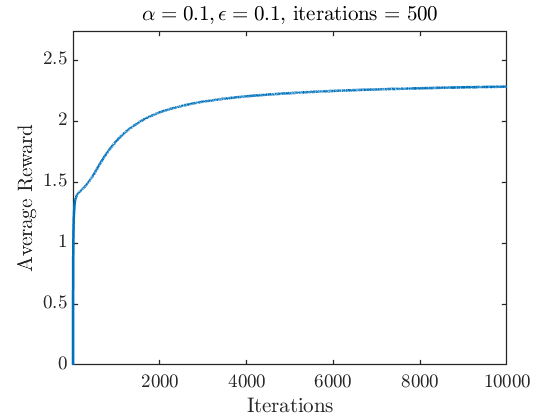
\includegraphics[width=\linewidth]{ex_2_5_fig_1a}
			\caption{$q_{*}(a)$ is stationary}
		\end{subfigure}
		\begin{subfigure}{0.45\textwidth}
			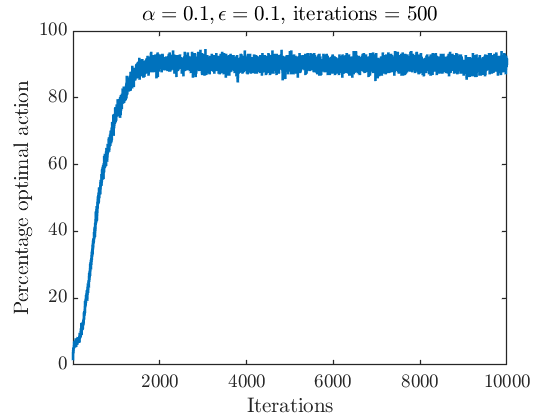
\includegraphics[width=\linewidth]{ex_2_5_fig_1b}
			\caption{$q_{*}(a)$ is stationary}
			\label{f1}
		\end{subfigure}
	\newline
		\begin{subfigure}{0.45\textwidth}
			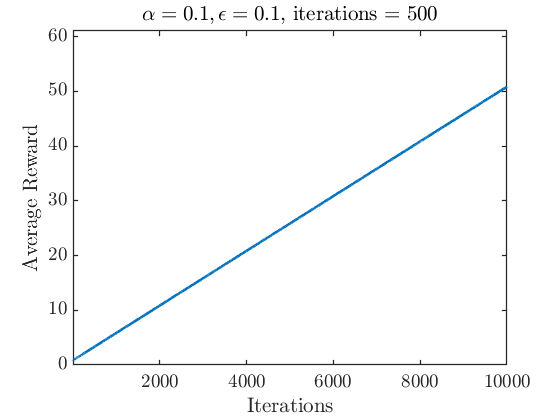
\includegraphics[width=\linewidth]{ex_2_5_fig_2a}
			\caption{$\mathbb{E}\left[ q_{*}(a) \right]$ increases by 0.01 on every timestep}
		\end{subfigure}
		\begin{subfigure}{0.45\textwidth}
			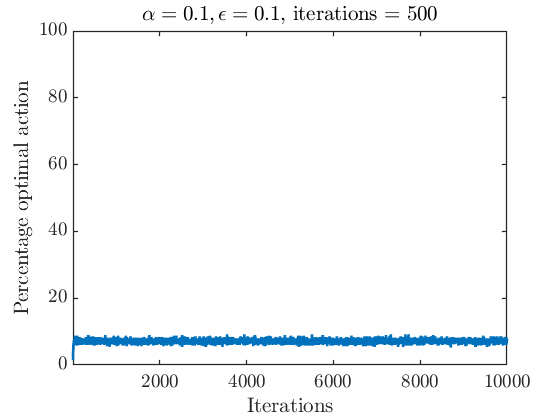
\includegraphics[width=\linewidth]{ex_2_5_fig_2b}
			\caption{$\mathbb{E}\left[ q_{*}(a) \right]$ increases by 0.01 on every timestep}
			\label{f2}
		\end{subfigure}
	\end{figure}
	From Figure~\ref{f1} and Figure~\ref{f2}, it can be seen that if $q_{*}(a)$ has a stationary distribution then the optimal action is chosen more and more as time progresses. However , in the non-stationary case, because the distribution of $q_{*}(a)$ is constantly changing, the percentage of times an optimal action is taken remains very low.
	%
	\subsection*{Exercise 2.6}
	\label{ss:2.6}
	\addcontentsline{toc}{subsection}{\nameref{ss:2.6}}
	All policies which `explore' in the beginning, as opposed to immediately exploiting its knowledge from the start will show spikes on initial timesteps. This is because as the policy explores the action space, it will invariably explore the action with highest expected return, among all other actions. This will cause the observed spike. However, due to the optimistic initial values, the policy will not stop at that action but rather continue to search through other actions to determine optimality - thus leading to the `dip' of the spike.
	%
	\subsection*{Exercise 2.7}
	\label{ss:2.7}
	\addcontentsline{toc}{subsection}{\nameref{ss:2.7}}
	Rearranging the terms for the recursive definition of $\bar{o}_n$, we get
	\begin{equation}
	\label{eq:e2.7_1}
	\bar{o}_n-\alpha = (1-\alpha)\bar{o}_{n-1}.
	\end{equation}
	We now consider the recursion equation of $Q_n$ with step size $\beta = \alpha/\bar{o}_n$.
	\begin{align*}
	Q_{n+1} &= Q_n + \beta_n (R_n - Q_n)\\
	&= (1-\beta_n)Q_n + \beta_n R_n\\
	&= \left(1-\frac{\alpha}{\bar{o}_n}\right)Q_n + \left( \frac{\alpha}{\bar{o}_n} \right)R_n\\
	\therefore \bar{o}_n Q_{n+1} &= (\bar{o}_n - \alpha)Q_n + \alpha R_n.
	\end{align*}
	We replace the value of $(\bar{o}_n-\alpha)$ from~\eqref{eq:e2.7_1} into the above.
	\begin{align*}
	\bar{o}_nQ_{n+1} = (1-\alpha)\bar{o}_{n-1}Q_n + \alpha R_n.
	\end{align*}
	Letting $\phi_k \ldef \bar{o}_{k-1}Q_k$ for all $k\in\mathbb{N}$, we get
	\begin{align*}
	\phi_{n+1} = (1-\alpha)\phi_n + \alpha R_n.
	\end{align*}
	This is similar to the recursion equation for $Q_n$ in the constant step-size case given as
	\begin{align*}
	Q_{n+1} &= (1-\alpha)Q_n + \alpha R_n\\
	&= (1-\alpha)^n Q_1 + \sum_{i=0}^{n-1} \alpha(1-\alpha)^i R_{n-1}.
	\end{align*}
	Thus, we can write the closed form solution of $\phi_n$ as
	\begin{align*}
	\phi_{n+1} &= (1-\alpha)^n \phi_1 + \sum_{i=0}^{n-1} \alpha(1-\alpha)^{i}R_{n-i}\\
	\therefore\bar{o}_nQ_{n+1} &= (1-\alpha)^n\phi_0 Q_1 + \sum_{i=0}^{n-1} \alpha(1-\alpha)^i R_{n-i}.
	\end{align*}
	However, noting that $\bar{o}_0 = 0$ by definition, we have $\phi_1 = \bar{o}_0 Q_1 = 0.Q_1 = 0$. Thus we get
	\begin{align*}
	\bar{o}_nQ_{n+1} = \sum_{i=0}^{n-1} \alpha(1-\alpha)^i R_{n-i},
	\end{align*}
	thereby proving that $Q_{n+1}$ is \emph{unbiased} by initial estimate $Q_1$.
	%
	\subsection*{Exercise 2.8}
	\label{ss:2.8}
	\addcontentsline{toc}{subsection}{\nameref{ss:2.8}}
	A `spike' is observed in the graph of average return around timestep 11 because this corresponds to the first timestep when the action with the highest average return (call this action $a'$) is chosen by the policy for the first time. \par\noindent
	However, after choosing $a'$, even though the value of $Q_t(a')$ increases, the upper confidence bound (UCB) term $c\sqrt{ \frac{\ln t}{N_t(a)} }$ for other actions $a$ increases when these actions are not selected. Thus the increase in the UCB term for other actions overpowers the increase in $Q_t(a')$ for action $a'$, and thus the policy keeps `exploring' and collecting lower rewards, rather than continuously perform action $a'$, leading to a `dip' in the average return graph. \par\noindent
	It should also be noted that for smaller values of $c$, the UCB term has less emphasis in choice of action, and therefore the spike will be less pronounced.
	\subsection*{Exercise 2.9}
	The sigmoid function $S(x)$ is defined as
	\begin{equation*}
	S(x) \ldef \frac{1}{1+e^{-x}}.
	\end{equation*}
	Suppose we only have 2 actions namely $a$ and $b$. Then the softmax distribution gives the probability of each of the actions as
	\begin{align*}
	P \{ A_t = a \} &= \frac{e^{H_t(a)}}{e^{H_t(a)} + e^{H_t(b)} }\\
	&= \frac{1}{1 + e^{H_t(b) - H_t(a)}}\\
	&= \frac{1}{1 + e^{-(H_t(a) - H_t(b))}}.\\
	P \{ A_t = b \} &= \frac{e^{H_t(b)}}{e^{H_t(a)} + e^{H_t(b)} }\\
	&= \frac{1}{1 + e^{-(H_t(b) - H_t(a))}}.
	\end{align*}
	As we can see, the probabilities for both actions $a$ and $b$ take form of a sigmoid function in the two action case.
	%
	\subsection*{Exercise 2.9}
	\label{ss:2.9}
	\addcontentsline{toc}{subsection}{\nameref{ss:2.9}}
	In case we are not told about the timestep on which case A or case B holds, we should treat the problem as a non-stationary bandit problem, and use any of the methods introduced in this chapter with a constant step size $\alpha$ for updating $Q_t(a)$.\par\noindent
	In case we know about the case on each timestep, we should maintain 4 $Q$ values. Calling the actions $a$ and $b$, the $Q$-values will be $Q_t^A(a)$, $Q_t^B(a)$, $Q_t^A(b)$, and $Q_t^B(b)$, and update them on each timestep according to whether the timestep falls under Case A or Case B.
	%
	\subsection*{Exercise 2.10}
	\label{ss:2.10}
	\addcontentsline{toc}{subsection}{\nameref{ss:2.10}}
	\begin{figure}[H]
		\centering
		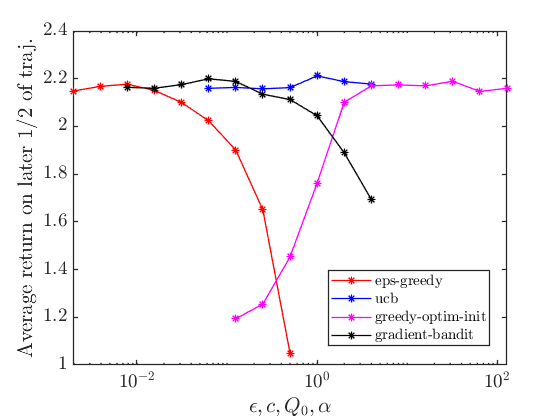
\includegraphics[width=0.5\linewidth]{ex_2_10_fig_1}
		\caption{Parameter study of various bandit algorithms.}
	\end{figure}
	%
	\subsection*{Improtant note: Gradient Bandits as Stochastic Gradient Ascent}
	\label{ss:gb-sga}
	\addcontentsline{toc}{subsection}{\nameref{ss:gb-sga}}
	In this section, we show how the gradient bandit algorithm can be derived from stochastic gradient ascent. The proof is taken verbatim from the textbook, except for trimming out some text and increasing clarity of presentation. Consider the preference $H_t(a)$ for action $a$. Its evolution can be characterized in terms of its effect on the epected reward $\mathbb{E}[R_t]$, which is given as
	\begin{align*}
	H_{t+1}(a) = H_t(a) + \alpha \frac{  \partial \mathbb{E} [R_t]}{\partial H_t(a)},
	\end{align*}
	where the expectation term $\mathbb{E} [R_t]$ can be expanded as
	\begin{equation*}
	\mathbb{E} [R_t] = \sum_{x} \pi_t(x) q_{*}(x), \;\; x\in\mathcal{A}.
	\end{equation*} 
	The partial derivative can be evaluated as
	\begin{align*}
	\frac{\partial \mathbb{E}[R_t]}{\partial H_t(a)} &= \frac{\partial}{\partial H_t(a)} \left[ \sum_{x} \pi_t(x)q_{*}(x) \right]\\
	&= \sum_{x} q_{*} (x) \frac{\partial \pi_t(x)}{\partial H_t(a)}\\
	&\stackrel{[r1]}{=} \sum_{x} (q_{*}(x) - B_t) \frac{\partial \pi_t(x)}{\partial H_t(a)}.
	\end{align*}
	The equality [r1] contains the term $B_t$ called \emph{baseline}, which can be any time-varying function not dependent on $x$. [r1] is a valid equality since $-B_t\sum_{x} \frac{\partial \pi_t(x)}{\partial H_t(a)} = 0$. This can be shown as
	\begin{align*}
	\sum_{x} \pi_t(x) = 1 \implies \frac{\partial}{\partial H_t(a)} \left[ \sum_{x} \pi_t(x) \right] = 0 \implies \sum_{x} \frac{\partial \pi_t(x)}{\partial H_t(a)} = 0 \stackrel{[r2]}{\implies} -B_t\sum_{x} \frac{\partial \pi_t(x)}{\partial H_t(a)} = 0,
	\end{align*}
	where in [r2], we multiplied the LHS and RHS of the preceding equality with $B_t$. \par\noindent
	Multiplying and dividing the RHS in [r1] with $\pi_t(x)$, we can represent the closed form of $\frac{\mathbb{E}[R_t]}{\partial H_t(a)}$ in the form of as expectation, as shown below.
	\begin{align*}
	\frac{\mathbb{E}[R_t]}{\partial H_t(a)} &= \sum_{x} \pi_t(x) (q_{*}(x) - B_t) \frac{\partial \pi_t(x)}{\partial H_t(a)}\frac{1}{\pi_t(x)}\\
	& \stackrel{[r3]}{=} \mathbb{E}_{A_t\in\mathcal{A}}\left[ (q_{*}(A_t) - B_t) \frac{\partial \pi_t(A_t)}{\partial H_t(a)}\frac{1}{\pi_t(A_t)} \right]\\
	& \stackrel{[r4]}{=} \mathbb{E}_{A_t\in\mathcal{A}}\left[ (q_{*}(A_t) - \bar{R}_t) \frac{\partial \pi_t(A_t)}{\partial H_t(a)}\frac{1}{\pi_t(A_t)} \right]\\
	& \stackrel{[r5]}{=} \mathbb{E}_{A_t\in\mathcal{A}}\left[ (R_t - \bar{R}_t) \frac{\partial \pi_t(A_t)}{\partial H_t(a)}\frac{1}{\pi_t(A_t)} \right].
	\end{align*}
	In the above, in [r2], we replace the term $x$ with the random variable $A_t$ over whose values the expectation is taken. In [r3], we chose $\bar{R}_t \ldef t^{-1}\sum_{i=1}^t R_t$ as our baseline $B_t$, and finally in [r4] we replace $q_{*}(A_t)$ with $R_t$ since $\mathbb{E} [ R_t \, \vert A_t = a] = q_{*}(a)$.\par\noindent
	We now find a closed form of $\frac{\partial \pi_t(A_t)}{\partial H_t(a)}$ which we will plug back into [r5]. Recall that in the gradient bandit algorithm, the action is chosen according to a softmax distribution given by  
	\begin{align*}
	\pi_t (x) = \frac{ \exp(H_t(x))}{ \sum_{y=1}^k \exp(H_t(y)) }.
	\end{align*}
	Letting $\mu \ldef  \sum_{y=1}^k \exp(H_t(y))$, we carry out the differentiation in the partial derivative using the quotient rule of differentiation as follows.
	\begin{align*}
	\frac{\partial \pi_t(x)}{\partial H_t(a)} &= \frac { \frac{\partial \exp(H_t(x)) }{ \partial H_t(a) }\mu - \exp(H_t(x)) \frac{\partial \mu}{\partial H_t(a)} }{\mu^2}\\
	&= \mathbbm{1}_{x=a}\frac{\exp(H_t(x))}{\mu} - \frac{ \exp(H_t(x)) \exp(H_t(a))}{\mu^2}\\
	&= \mathbbm{1}_{x=a}\pi_t(x) - \pi_t(x)\pi_t(a) = \pi_t(x) \left[ \mathbbm{1}_{x=a} - \pi_t(a) \right].
	\end{align*}
	Pluging the above result back in [r5], we get
	\begin{align*}
	\frac{\mathbb{E}[R_t]}{\partial H_t(a)} &= \mathbb{E}_{A_t\in\mathcal{A}}\left[ (R_t - \bar{R}_t) \pi_t(A_t) (\mathbbm{1}_{A_t=a}-\pi_t(a))\frac{1}{\pi_t(A_t)} \right]\\
	&\stackrel{[r6]}{=} \mathbb{E}_{A_t\in\mathcal{A}}\left[ (R_t - \bar{R}_t) (\mathbbm{1}_{A_t=a}-\pi_t(a)) \right].
	\end{align*}
	In the gradient bandit algorithm, we update the term using the formula inside the expectation in [r6] (as an approximation), thereby proving that the gradient bandit update rule is derived from stochastic gradient ascent.
	\newpage
	%
	\section{Chapter 3}
	%
	\subsection*{Exercise 3.1}
	\label{ss:3.1}
	\addcontentsline{toc}{subsection}{\nameref{ss:3.1}}
	Three applications are presented as follows.
	\begin{enumerate}
		\item \textbf{AI chess player:} We can design an autonomous agent that learns to play chess using reinforcement learning.
		\begin{itemize}
			\item \emph{State:} Position of various pieces on the chess board.
			\item \emph{Actions:} Agent can move each of its pieces to a legal position, and declare checkmate.
			\item \emph{Reward:} $+1$ when an opponent piece is knocked out, $-1$ when an own piece is knocked out, $+M$ for checkmate, where $M$ is a large number.
		\end{itemize}
		\item \textbf{Autonomous driving agent} We can design an agent which can drive a car autonomously in the real world, like a Tesla car.
		\begin{itemize}
			\item \emph{State:} Input from the car's sensors like camera, LIDAR, etc.
			\item \emph{Actions:} Inputs to steering, brake, and accelerator.
			\item \emph{Reward:} The reward can be defined as a two-argument function $r(t',\mathbf{d})$, where $t'$ is the remaining time to reach destination, and $\mathbf{d}$ is a vector that provides the vehicle's distance from other vehicles and obstacles. $r$ should in general be decreasing in $t'$ and increasing in each dimension of $\mathbf{d}$.
		\end{itemize}
		\item \textbf{Adaptive beam steering} Nowadays, there are multiple antennae which can electronically steer beams in order to provide better signal reception at the user. We consider an antenna which steers beams in 2D and uses reinforcement learning to reckon the optimal steering angle.
		\begin{itemize}
			\item \emph{State:} Current direction in which beam is focused.
			\item \emph{Action:} Angle $\theta$ by which to steer the beam.
			\item \emph{Reward:} SNR (signal to noise ratio) received at user terminal.
		\end{itemize}
	\end{enumerate}
	%
	\subsection*{Exercise 3.2}
	\label{ss:3.2}
	\addcontentsline{toc}{subsection}{\nameref{ss:3.2}}
	One of the cases where MDP framework might be insufficient is where the reward might he a high-dimensional vector instead of a scalar. In this case, we cannot calculate which reward $\mathbf{r}$ or $\mathbf{r}'$ may be `better', since for some indices $\mathbf{r}$ would be greater than $\mathbf{r}'$ and in other indices it could be smaller. Thus we would require additional context for determining optimality of received rewards. 
	%
	\subsection*{Exercise 3.3}
	\label{ss:3.3}
	\addcontentsline{toc}{subsection}{\nameref{ss:3.3}}
	The correct interface between the environment and action in this case would be at the steering wheels, brake, and accelerator. This is because RL stipulates that the `agent' should be the one which has complete control authority over its actions, and in this case, it is fair to assume that complete control authority over driving the car can be achieved by manipulating the steering wheel, accelerator, and brake pedal. Going to a `lower' level than this, e.g. torques on the wheels, might make planning  for activities like driving to a specific location difficult, while any `higher' level, such as in the brain of a driver, would make the action space of the MDP so large that it would become intractable to use in a RL problem.
	%
	\subsection*{Exercise 3.4}
	\label{ss:3.4}
	\addcontentsline{toc}{subsection}{\nameref{ss:3.4}}
	Note that we denote the state space \{High, Low\} as $\{H,L\}$, the action space \{Search, Wait, Recharge\} as $\{S,W,R\}$ and the reward space $\{r_{search},r_{wait},r_{penalty},0\}$ as $\{s,w,p,0\}$, where $r_{penalty}=-3$ is the reward (penalty) if the robot has to be manually recovered due to low charge.
	\begin{center}
	\begin{tabular}[H]{|c|c|c|c|c|}
		\hline
		$s$ & $a$ & $s'$ & $r$ & $p(s',r | s,a)$\\
		\hline\hline
		$H$ & $S$ & $H$ & $s$ & $\alpha$\\
		\hline
		$H$ & $S$ & $L$ & $s$ & $1-\alpha$\\
		\hline
		$L$ & $S$ & $H$ & $p$ & $1-\beta$\\
		\hline
		$L$ & $S$ & $L$ & $s$ & $\beta$ \\
		\hline
		$H$ & $W$ & $H$ & $w$ & $1$\\
		\hline
		$L$ & $W$ & $L$ & $w$ & $1$\\
		\hline
		$L$ & $R$ & $H$ & $0$ & $1$\\
		\hline
	\end{tabular}
	\end{center}
	%
	\subsection*{Exercise 3.5}
	\label{ss:3.5}
	\addcontentsline{toc}{subsection}{\nameref{ss:3.5}}
	Let $\mathcal{S}$ be the space of all non-terminal states, $\mathcal{R}$ be the space of all rewards, and $s^+$ be the terminal state. Then (3.3) can be modified for episodic tasks as
	\begin{align*}
	\sum_{s\in\mathcal{S}} \sum_{r\in\mathcal{R}} p(s',r | s,a) + \sum_{r\in\mathcal{R}} p(s^+,r | s,a) = 1.
	\end{align*}
	%
	\subsection*{Exercise 3.6}
	\label{ss:3.6}
	\addcontentsline{toc}{subsection}{\nameref{ss:3.6}}
	In case of an episodic formulation, the return on any timestep $t$ is given as $G_t = -\gamma^{K_t}$ where $K_t$ is a random variable denoting the number of timesteps form $t$ when the first failure occurs. Because we are in an episodic setting, $K_t$ is also the final timestep of any episode.\par\noindent
	In the continuing task formulation, the return is given as $G_t = -\gamma^{K^1_t} - \gamma^{K^2_t} - \gamma^{K^3_t} - \cdots$ where $K^i_t$ is a random variable denoting the time to $i$th failure fom timestep $t$. Since in the episodic formulation the state is automatically reset after any failure, the return on any timestep $t$ considers the possibilities of all failures that can happen in the future. Note that due to causality, $K^{i+1}_t > K^i_t$ for every timestep $t$ for all $i\in\mathbb{N}$.
	%
	\subsection*{Exercise 3.7}
	\label{ss:3.7}
	\addcontentsline{toc}{subsection}{\nameref{ss:3.7}}
	If the robot's performance in escaping the maze is not improving after a while, the most probable reason would be that the reward scheme is not 'motivating' the learning agent sufficiently to escape the maze. One of the solutions is to increase the terminal reward to $+M$ where $M>0$ is a very large value, in order to increase the incentive on the terminal state. Another solution would be to assign a penalty of $-1$ to all timesteps where the exit of the maze is not reached. This will place a negative reward on the time elapsed before the agent escapes the maze, thereby incentivizing it to do so.
	%
	\subsection*{Exercise 3.8}
	\label{ss:3.8}
	\addcontentsline{toc}{subsection}{\nameref{ss:3.8}}
	The various values of $G_t$ can be calculated as follows, starting backward from $G_5$, whose value is $0$ since $T=5$ is the final timestep of the episode.
	\begin{align*}
	G_5 &= 0,\\
	G_4 &= R_5 + \gamma G_5 = 2 + (0.5)(0) = 2,\\
	G_3 &= R_4 + \gamma G_4 = 3 + (0.5)(2) = 4,\\
	G_2 &= R_3 + \gamma G_3 = 6 + (0.5)(4) = 8,\\
	G_1 &= R_2 + \gamma G_2 = 2 + (0.5)(8) = 6,\\
	G_0 &= R_1 + \gamma G_1 = -1 + (0.5)(6) = 2.
	\end{align*}
	%
	\subsection*{Exercise 3.9}
	\label{ss:3.9}
	\addcontentsline{toc}{subsection}{\nameref{ss:3.9}}
	We will first calculate $G_1$ and then use its value to calculate $G_0$. Since $R_t = 7$ for $t\geq 2$, we have
	\begin{align*}
	G_1 &= R_2 + \gamma R_3 + \gamma^2 R_4 + \cdots\\
	&= 7 + \gamma.7 + \gamma^2.7 + \cdots\\
	&= 7(1 + \gamma + \gamma^2 + \cdots)\\
	&\stackrel{[r7]}{=} \frac{7}{1-\gamma} = \frac{7}{1-0.9} = 70. 
	\end{align*}
	In [r7] we have used equation (3.10) from the textbook. We can now calculate $G_0$ as
	\begin{align*}
	G_0 &= R_1 + \gamma G_1\\
	&= 2 + (0.9)(70) = 65.
	\end{align*}
	%
	\subsection*{Exercise 3.10}
	\label{ss:3.10}
	\addcontentsline{toc}{subsection}{\nameref{ss:3.10}}
	We want to prove that
	\begin{align}
	\sum_{k=0}^{\infty} \gamma^k = \frac{1}{1-\gamma}, \;\; \forall 0\leq\gamma<1.
	\label{eq:e3.9_1}
	\end{align}
	The proof of~\eqref{eq:e3.9_1} is as follows: we define the partial sum $S_k$ as 
	\begin{align*}
	S_k &\ldef \sum_{j=0}^{k} \gamma^j
	= 1 + \gamma + \gamma^2 + \cdots + \gamma^k.
	\end{align*}
	Now we carry out some algebraic manipulations on the partial sum $S_k$ as given below.
	\begin{align*}
	\gamma S_k &= \gamma \sum_{j=0}^k \gamma^j
	= \sum_{j=1}^{k+1} \gamma^j.\\
	\therefore \;\; S_k - \gamma S_k &= \sum_{j=0}^k \gamma^j - \sum_{j=1}^{k+1} \gamma^j
	= 1 - \gamma^{k+1}.\\
	\therefore \;\; S_k &= \frac{1 - \gamma^{k+1}}{1-\gamma}.
	\end{align*}
	Using the fact that $\lim\limits_{k\rightarrow\infty} S_k = \sum_{k=0}^{\infty} \gamma^k$ and that $\lim\limits_{k\rightarrow\infty} \gamma^{k+1} = 0$ for $|\gamma|<1$, we have
	\begin{align*}
	\sum_{k=0}^{\infty} \gamma^k = \lim\limits_{k\rightarrow\infty} \frac{1-\gamma^{k+1}}{1-\gamma} = \frac{1}{1-\gamma},
	\end{align*}
	thereby completing the proof.
	%
	\subsection*{Exercise 3.11}
	\label{ss:3.11}
	\addcontentsline{toc}{subsection}{\nameref{ss:3.11}}
	We have to find out a closed form expression for $\mathbb{E} \left[ R_{t+1} | S_t = s \right]$ in terms of the MDP dynamics $p(s',r|s,a)$ and the policy $\pi(a|s)$. We first use the law of total expectation to expand the aforementioned expectation term as
	\begin{align*}
	\mathbb{E}\left[ R_{t+1} | S_t = s \right] &= \mathbb{E} \left[ \mathbb{E} \left[ R_{t+1} | S_t = s, A_t = a \right] | S_t = s\right]\\
	&= \mathbb{E} \left[ \sum_{r\in\mathcal{R}} r p(r | s,a) \big| S_t = s \right]\\
	&= \mathbb{E} \left[ \sum_{r\in\mathcal{R}} r \sum_{s'\in\mathcal{S}}p(s',r| s,a) \big| S_t = s \right].
	\end{align*}
	Noting that the above expectation is to be taken over all actions $a\in\mathcal{A}(s)$, we derived the closed form of $\mathbb{E}\left[ R_{t+1} | S_t = s \right]$ in terms of $p$ and $\pi$ as
	\begin{align*}
	\mathbb{E}\left[ R_{t+1} | S_t = s \right] &= \mathbb{E}_{a\in\mathcal{A}(s)} \left[ \sum_{r\in\mathcal{R}} 
	\sum_{s'\in\mathcal{S}} r p(s',r| s,a) \big| S_t = s \right]\\
	&= \sum_{a\in\mathcal{A}(s)} \pi(a|s) \sum_{r\in\mathcal{R}} 
	\sum_{s'\in\mathcal{S}} r p(s',r| s,a).
	\end{align*}
	%
	\subsection*{Exercise 3.12}
	\label{ss:3.12}
	\addcontentsline{toc}{subsection}{\nameref{ss:3.12}}
	Using the law of total expectations, we see that
	\begin{align*}
	v_{\pi}(s) = \mathbb{E}_{\pi} \left[ G_t | S_t = s \right] &= 
	\mathbb{E}_{\pi} \left[ \mathbb{E}_{\pi} \left[ G_t | S_t = s, A_t = a \right] | S_t = s \right]\\
	&= \mathbb{E}_{\pi} \left[ q_{\pi}(s,a) | S_t = s \right] = \sum_{a\in\mathcal{A}(s)} \pi(a|s)q_{\pi}(a,s).
	\end{align*}
	%
	\subsection*{Exercise 3.13}
	\label{ss:3.13}
	\addcontentsline{toc}{subsection}{\nameref{ss:3.13}}
	Using the definition of $q_{\pi}(s,a)$, we see that
	\begin{align*}
	q_{\pi}(s,a) &= \mathbb{E}_\pi \left[ G_t | S_t = s, A_t = a \right] \\
	&= \mathbb{E}_\pi \left[ R_t + \gamma G_{t+1} | S_t = s, A_t = a \right] \\
	&\stackrel{[r8]}{=} \mathbb{E}_\pi \left[ R_t + \gamma \mathbb{E}_\pi \left[ G_{t+1} | S_{t+1} = s',S_t = s,A_t = a \right] | S_t = s, A_t = a \right]\\
	&\stackrel{[r9]}{=} \mathbb{E}_\pi\left[ R_t + \gamma \mathbb{E}_\pi \left[ G_{t+1} | S_{t+1} = s' \right] | S_t = s, A_t = a \right]\\
	&= \mathbb{E}_\pi \left[ R_t + \gamma v_{\pi} (s') | S_t = s, A_t = a \right]\\
	&= \sum_{r\in\mathcal{R}} \sum_{s'\in\mathcal{S}} p(s',r|s,a) \left[ r + \gamma v_{\pi} (s') \right].
	\end{align*}
	Note that in the above calculations, in [r8] we use the law of total expectations to expand the inner expectation, while in [r9] we have used the fact that $G_t$ follows Markov property.
	%
	\subsection*{Important note: Bellman Recusion}
	\label{ss:bell-rec}
	\addcontentsline{toc}{subsection}{\nameref{ss:bell-rec}}
	From the results of Exercise 3.12 and Exercise 3.13, we can derive a formula to calculate $v_{\pi}(s)$ in terms of $v_{\pi}(s')$.
	\begin{align*}
	v_{\pi}(s) &= \sum_{a\in\mathcal{A}(s)} \pi(a|s)q_{\pi}(a,s)\\
	&= \sum_{a\in\mathcal{A}(s)} \pi(a|s)\sum_{r\in\mathcal{R}} \sum_{s'\in\mathcal{S}} p(s',r|s,a) \left[ r + \gamma v_{\pi} (s') \right].
	\end{align*} 
	The above formula is called the \textbf{Bellman Recursion Equation}.
	%
	\subsection*{Exercise 3.14}
	\label{ss:3.14}
	\addcontentsline{toc}{subsection}{\nameref{ss:3.14}}
	Let the center state be denoted by $c$. Let the action space be denoted by $\{ N,S,E,W \}$, which respectively represent the action of going north, south, east, and west. Corresponding to taking these actions, let the resulting states be denoted as $\{ c^N,c^S,c^E,c^W \}$. Furthermore, note that $\pi(N|c)=\pi(S|c)=\pi(E|c)=\pi(W|c)=0.25$ as mentioned in the book. Lastly, the only reward that can be gained by any action while on $c$ is 0, and therefore $p(c^N,0|c,N)=p(c^S,0|c,S)=p(c^E,0|c,E)=p(c^W,0|c,W)=1$. The Bellman recursion in this case is given as
	\begin{align*}
	v_{\pi}(c) &= \pi(N|c)\left( \gamma v_{\pi} (c^N) \right) + \pi(S|c)\left( \gamma v_{\pi} (c^S) \right) + \pi(E|c)\left( \gamma v_{\pi} (c^E) \right) + \pi(W|c)\left( \gamma v_{\pi} (c^W) \right)\\
	&= (0.25)(0.9)\left( 2.3 + 0.4 -0.4 + 0.7 \right) =0.675 \approx 0.7 = v_{\pi}(c).
	\end{align*}
	%
	\subsection*{Exercise 3.15}
	\label{ss:3.15}
	\addcontentsline{toc}{subsection}{\nameref{ss:3.15}}
	Let $v_{\pi}^c$ represent the value function of states when a constant $c$ is added to all the reward values. Correspondingly, let $G_t^c$ represent the infinite horizon discounted reward when $c$ is added to all rewards.
	We have
	\begin{align*}
	G_t^c &= (R_{t+1}+c) + \gamma(R_{t+2}+c) + \gamma^2(R_{t+3}+c)+\cdots\\
	&= \left( R_{t+1} + \gamma R_{t+2} + \gamma^2 R_{t+3} + \cdots \right) + c \left( 1 + \gamma + \gamma^2 + \cdots \right)\\
	&= G_t + \frac{c}{1-\gamma}.
	\end{align*}
	By the definition of $v_{\pi}^c(s)$, we have
	\begin{align*}
	v_{\pi}^c(s) = \mathbb{E}_{\pi} \left[ G_t + \frac{c}{1-\gamma} \big| S_t = s \right] = \mathbb{E}_{\pi} \left[ G_t | S_t = s \right] + \frac{c}{1-\gamma} = v_{\pi}(s) + \frac{c}{1-\gamma}.
	\end{align*}
	Thus, adding a constant c to all the rewards adds a constant of $\frac{c}{1-\gamma}$ to all the state values.
	% 
	\subsection*{Exercise 3.16}
	\label{ss:3.16}
	\addcontentsline{toc}{subsection}{\nameref{ss:3.16}}
	Using the notation from~\nameref{ss:3.15}, we can expand $G_t^c$ in the episodic case as
	\begin{align*}
	G_t^c &= (R_{t+1}+c) + \gamma(R_{t+2}+c) + \gamma^2 (R_{t+3}+c) + \cdots + \gamma^{T-(t+1)}(R_{T} + c)\\
	&= \left(R_{t+1} + \gamma R_{t+2} + \cdots + \gamma^{T-(t+1)}R_{T} \right) + c\left(1+\gamma+\cdots+\gamma^{T-(t+1)} \right)\\
	&= G_t + \frac{c(1-\gamma^{(T-t)})}{1-\gamma}.
	\end{align*}
	Letting $\phi(T) \ldef \frac{c(1-\gamma^{(T-t)})}{1-\gamma}$, we see that $v_\pi^c(s) = v_\pi(s) + \phi(T)$ for all states $s\in\mathcal{S}$ in the episodic case. Furthermore, note that $\phi(T)$ is \emph{increasing} in $T$ since $\frac{\partial \phi(T)}{\partial T} = \frac{c\gamma^{(T-t)}\log(1/\gamma)}{1-\gamma}>0$ for all $t\geq T$. Thus adding constant $c$ to all the rewards in the episodic case results in addition of the factor $phi(T)$ to the return $G_t$. Since $\phi(T)$ is increasing in $T$, it means that the agent will have an incentive to take a longer amount of time to complete the task in any given episode.
\end{document}